\chapter{Experiments}\label{experiments}

The goal of the experiments is to evaluate the word vector quality. First, we briefly describe the data, preprocessing and evaluation metrics. Next, we describe the testing environments (hardware and software). Moreover, the baseline methods are outlined. Furthermore, the implemented HPV hierarchies are described, and the possible hyperparameters will be outlined. Finally, the results will be shown.

\section{Experimental Setup and Data}\label{experimental-setup-and-data}

\subsection{IMDB Dataset}\label{imdb-dataset}

The Internet Movie Database (IMDB) dataset is a collection of movie reviews which have been written and rated by people. Each movie review consists of a text, which, in turn, consists of some sentences and has one or multiple paragraphs.

Additionally, half of the movie ratings have a rating $r \in [1,\ 10] \subseteq \mathbb{N}$, where a higher rating indicates that the reviewer likes the movie better. Furthermore, the movie ratings are divided into \emph{negative ratings} (numeric rating of 1, 2, 3 or 4) and \emph{positive ratings} (numeric rating of 7, 8, 9 or 10). \emph{Neutral ratings} with a numeric rating of 5 or 6 have been excluded from the dataset. The task is to perform sentiment analysis on the movie reviews: for a given review text, predict if the sentiment is positive or negative.

Besides the rated reviews, the other half of the reviews do not contain a rating and thus can only be used to learn the word embeddings, as we will see later. The distribution of the 100'000 movie rating can be seen in Figure~\ref{fig:5:movie-ratings-distribution}. More detailed information about the dataset can be found in~\cite{Maas2011}.

\begin{figure}
	\centering
	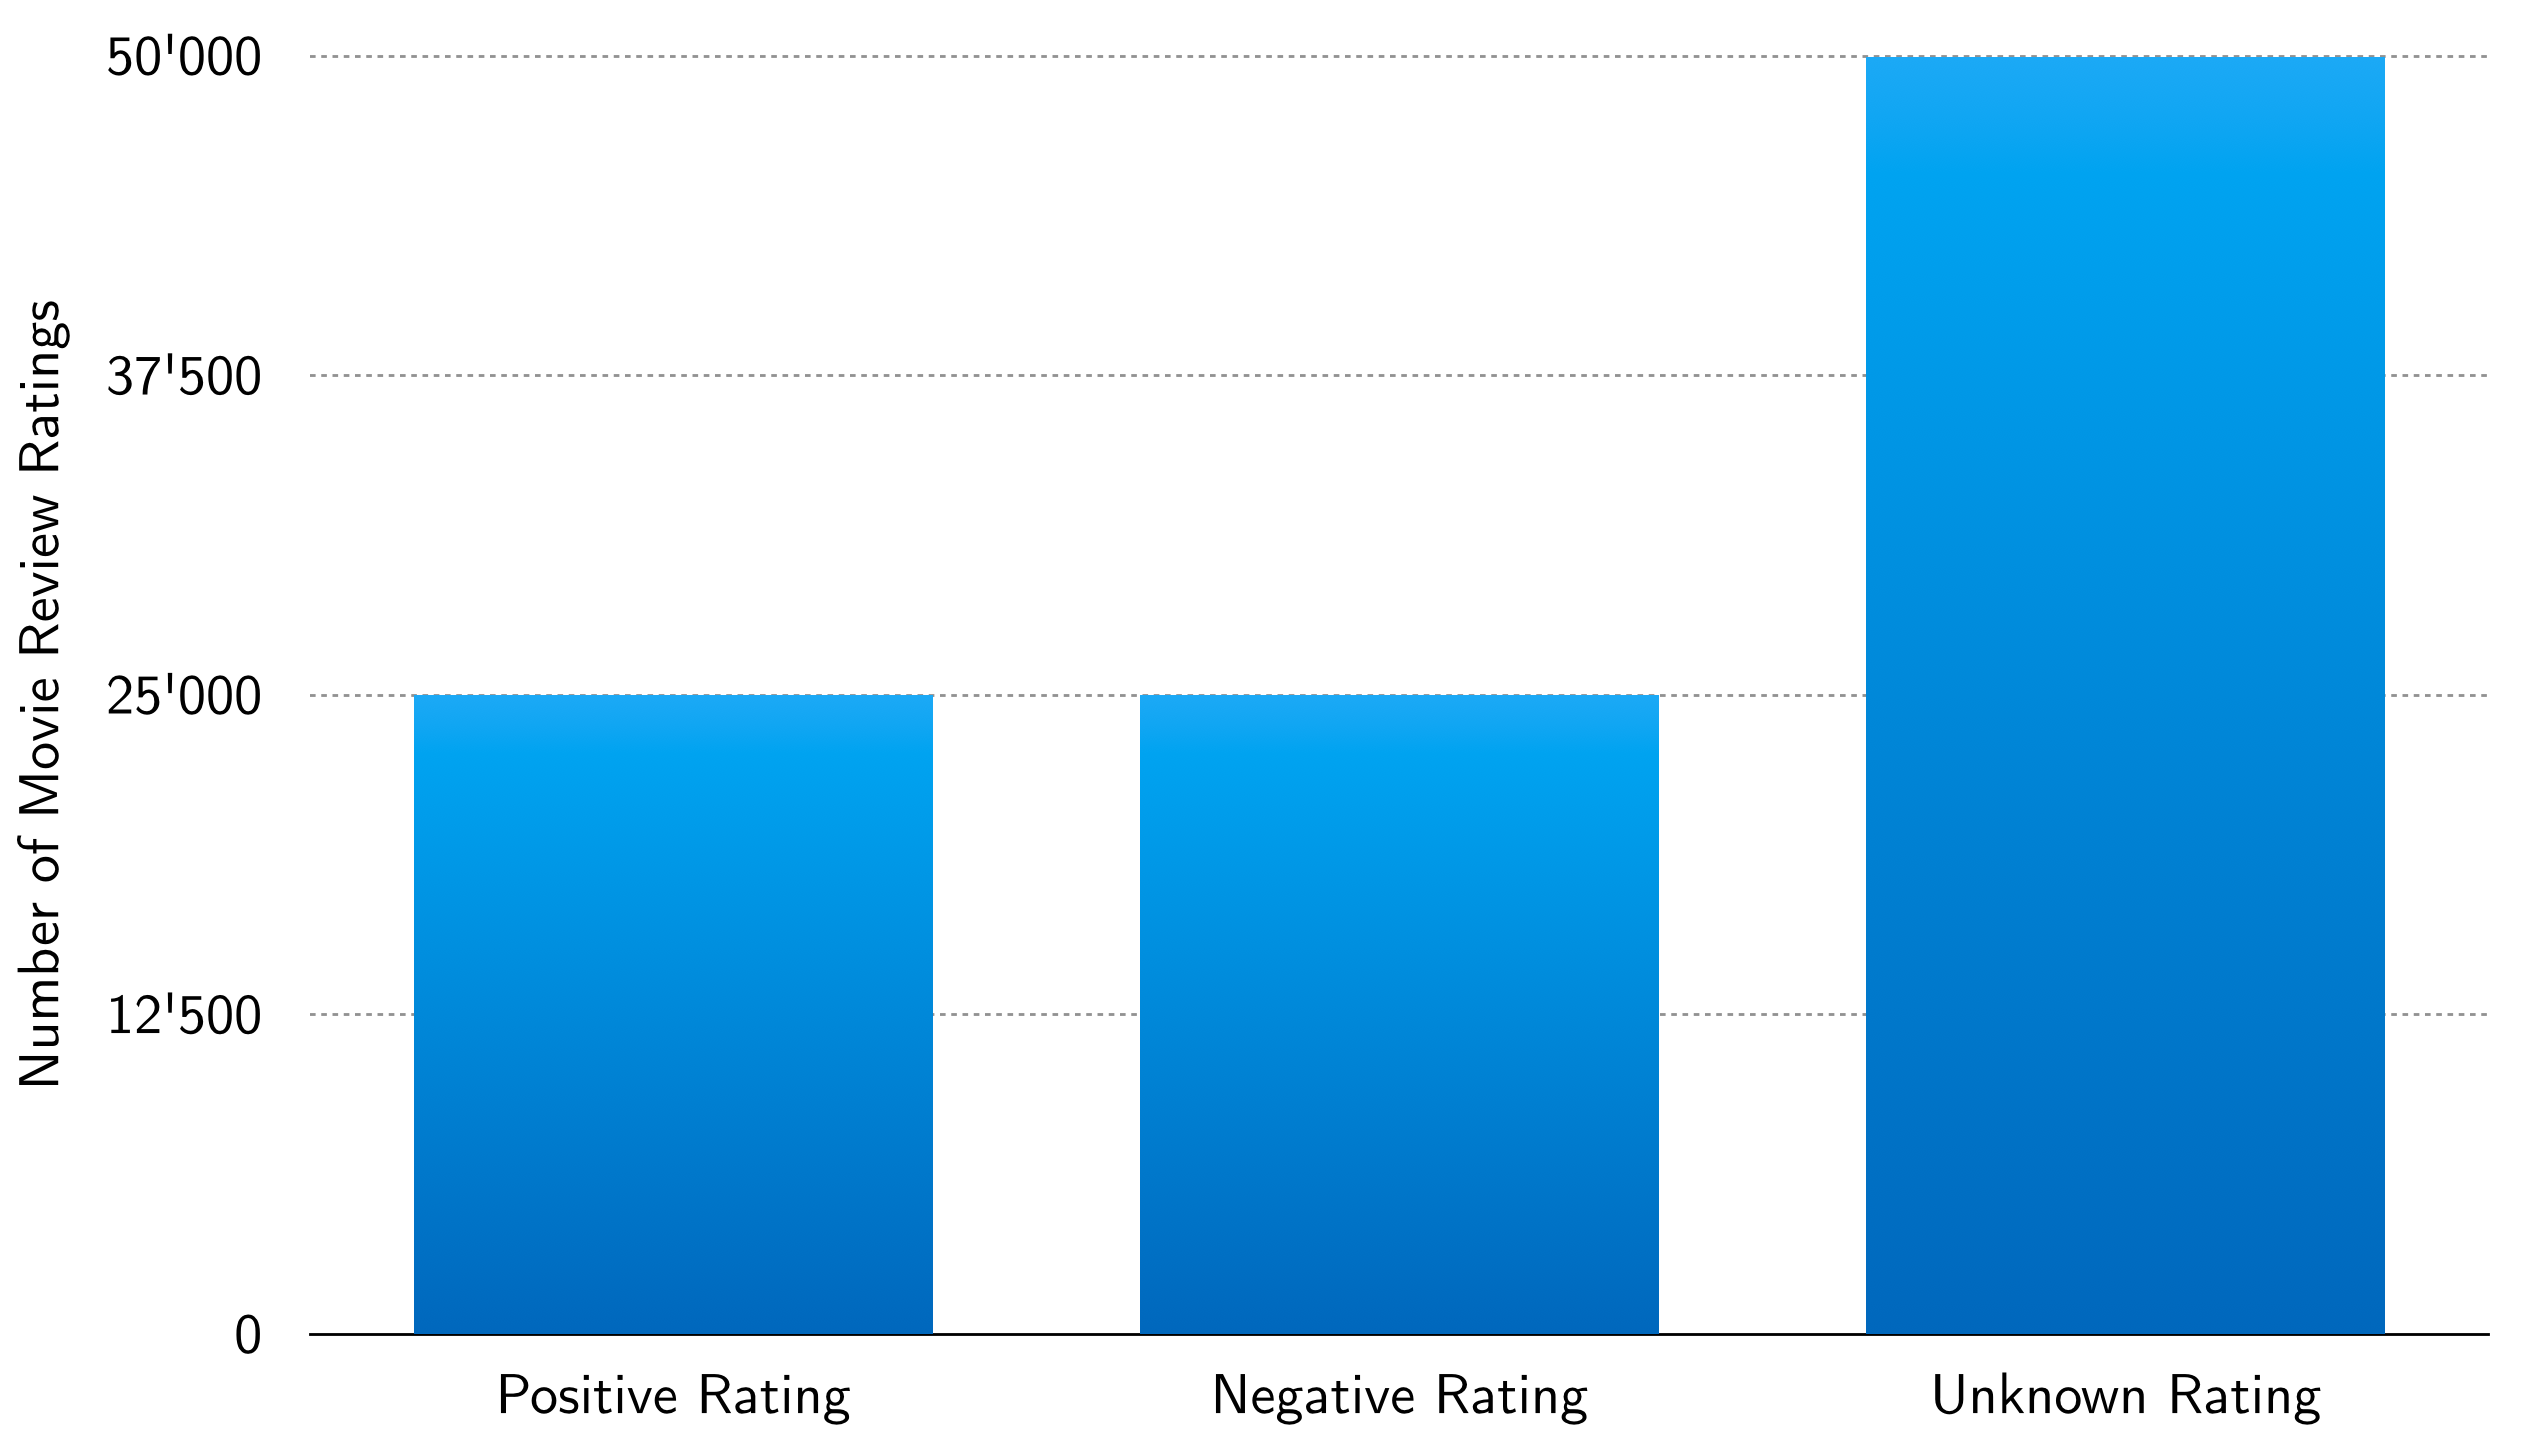
\includegraphics[width=1.0\textwidth]{5experiments/movie-ratings-distribution.png}
	\caption{The movie review ratings consist of an equal amount of positive and negative ratings. For half of the dataset, the rating is unknown.}
	\label{fig:5:movie-ratings-distribution}
\end{figure}


\subsection{Preprocessing}\label{preprocessing}

Preprocessing of text can lead to significant differences in the outcome of the results. Additionally, it can also help to reduce computational complexity, for example by removing invalid characters, which would be used as words, or by converting some similar characters to one general character. However, preprocessing is not the focus of this master thesis, and is therefore only applied limitedly.

First, different single quote symbols (for example ', ", `) are consolidated, and so are different double quote symbols. Next, frequently used HTML tags are converted to text symbols. Furthermore, common smilies are replaced by text symbols. Finally, punctuation, brackets, and commonly used special characters (for example dollar, hashtag) are replaced by text symbols. Other invalid symbols and uncommonly used characters are removed from the text. Finally, all text is converted to lowercase.

\subsection{Software}\label{software}

The original implementation by Mikolov only works for Word2vec, and would have to be extended to work with Doc2vec. Furthermore, this implementation is written in pure C, and is therefore difficult to modify, extend, and interact with.

There exist many implementations for Doc2vec. One of the fastest, if not the fastest implementation, is Gensim\footnote{\url{https://radimrehurek.com/gensim/}}. Furthermore, the implementation has a well-defined and simple interface to Python\footnote{\url{https://www.python.org/}}, and is well documented. For these reasons, Gensim was chosen as a library for the paragraph vector calculation. The exact versions are 3.4.3 for Python, and 0.12.1 for Gensim. The source code produced in the course of this thesis project can be found here\footnote{\url{https://github.com/lukaselmer/hierarchical-paragraph-vectors}}.

\subsection{Distributed Implementation}\label{distriubted-implementation}

To run a large amount of experiments and to record the results, the experiments needed to be run on a cluster. Thus, an implementation, which can distribute jobs and record results, was required. One job that consists of the parameters described below is executed on exactly one node, and is run through the whole dataset. Thus, the computation is not distributed in the traditional map-reduce way.

Running one batch of experiments works as follows: on one central server, the experiments are scheduled. Then, a client requests the parameters for one experiment to run, runs the experiment with these parameters, and submits the result to the central server. This process is executed as long as there are scheduled experiments. An overview of the architecture can be found in Figure~\ref{fig:5:architecture}.

\begin{figure}
	\centering
	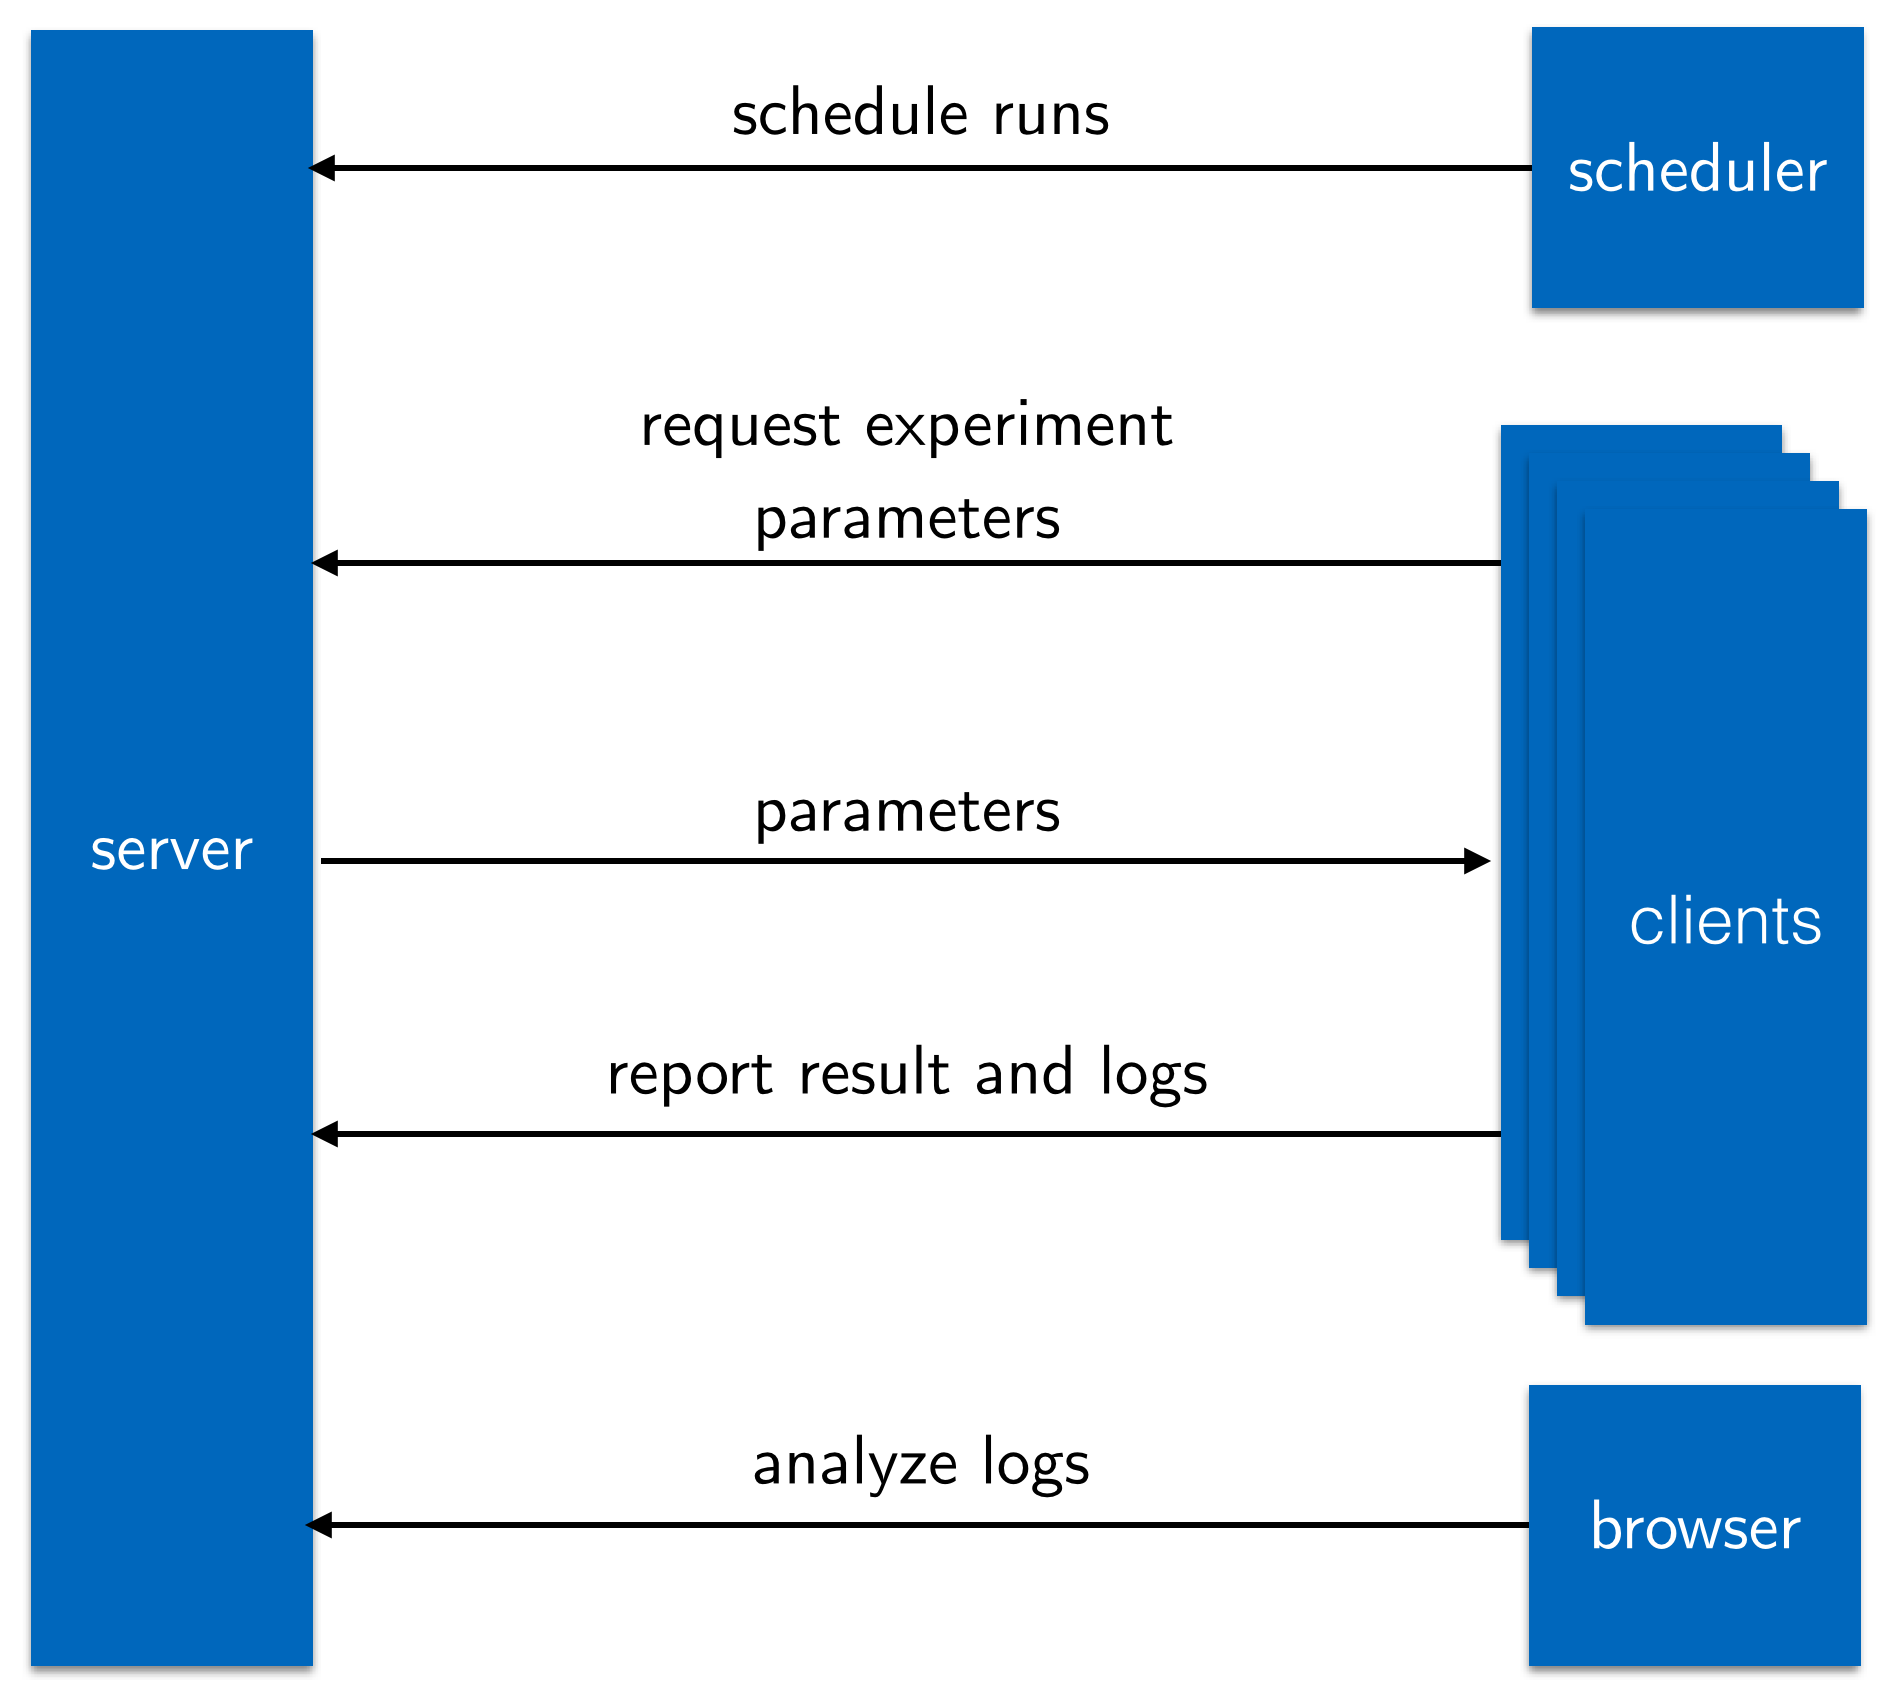
\includegraphics[width=0.7\textwidth]{5experiments/architecture.png}
	\caption{Architectural overview of the distributed implementation. The tiers communicate via HTTPS and JSON.}
	\label{fig:5:architecture}
\end{figure}

The central server is implemented in Ruby on Rails\footnote{\url{https://github.com/lukaselmer/simple-job-runner}}. In addition to the scheduling and result collection, the server also implements an interface to analyze the results and to generate charts. The client is implemented in Python, see~\ref{software}. Multiple clients request, run and submit experiments concurrently.

\subsection{Hardware}\label{hardware}

The software was developed on an ``Apple MacBook Pro, Core i7 2.8 (I7-4980HQ), 15-Inch, Mid-2014, Dual Graphics'', model id ``MacBookPro11,3''\footnote{\url{http://www.everymac.com/systems/apple/macbook_pro/specs/macbook-pro-core-i7-2.8-15-dual-graphics-mid-2014-retina-display-specs.html}}. Also, the performance tests in~\ref{5:execution-speed-and-memory-usage} have been conducted on this laptop. The operating system of the laptop was OS X Yosemite 10.10.5.

The restricted and unrestricted best configuration experiments in~\ref{5:accuracy} have been executed on 8 nodes of the DCO cluster at ETH\@. Each machine has 16 physical cores and 128 GB of physical RAM\@. The operating system of the servers was Fedora 21\footnote{\url{https://getfedora.org/}}.

\section{Evaluation Metrics}\label{evaluation-metrics}

Recall that the dataset is balanced between positive and negative ratings. Therefore, a random estimator would guess the sentiment of 50\% of the ratings correctly. The balanced dataset allows us to use accuracy as the first evaluation metric. We use the following definition to calculate the mean accuracy from the predicted reviews $R$.
\begin{displaymath}
\text{accuracy} = \frac{1}{\dim(R)} \sum_{r \in R} \begin{dcases*}
1& when $r_{\text{predicted sentiment}}$ = $r_{\text{actual sentiment}}$\\
0& otherwise
\end{dcases*}
\end{displaymath}
Note that this is a binary classification task.

The second and third evaluation metrics are training speed (computational complexity) and memory footprint which are measured empirically. The training speed is calculated by measuring the time from starting one training epoch until the training epoch has ended. Here, it is important to note that during the test, only one active program is being run on the machine, and no other computationally intensive programs are being run in the background. The memory footprint is measured by the size of a file to which the model is serialized.

\section{Baseline Methods}\label{baseline-methods}

There are two methods which draw a baseline to compare HPV to. The first baseline is to generate the word embeddings by using the commonly used term frequency - inverse document frequency (TF--IDF) method \cite{Rajaraman2011}. For the TF--IDF vectors, the features are ordered by term frequency across the corpus, and only the top $n$ features are used to get a low-dimensional vector. More details about the implementation can be found in \ref{appendix:tf-idf}.

The second baseline method is the standard implementation of Doc2vec provided by Gensim. As we will see, the same hyperparameters are used for the baseline and the HPV enhanced implementation.

Both baseline methods use the same classifier as the HPV implementations, which is a support vector classifier (SVC), see Table ~\ref{tab:parameters}.

\section{Implemented HPV Hierarchies}\label{implemented-hpv-hierarchies}

As we have seen before, there are two directions from which hierarchies can be obtained (upwards and downwards). Let us first investigate the upwards direction and thereafter continue with the downwards direction.

\begin{table}
	\centering
	\caption{Overview of the implemented hierarchies.}
	\label{tab:implemented-hpv-hierarchies}
	\begin{tabular}{ll}
		\toprule
		\emph{Abbreviation}& \emph{Hierarchies}\tabularnewline
		\midrule
		NO-HPV& None\tabularnewline
		HPV-TOP& Topics\tabularnewline
		HPV-TOP-PAR& Topics, Paragraphs\tabularnewline
		HPV-TOP-PAR-SENT& Topics, Paragraphs, Sentences\tabularnewline
		HPV-PAR& Paragraphs\tabularnewline
		HPV-PAR-SENT& Paragraphs, Sentences\tabularnewline
		HPV-PAR-SENT-SUB& Paragraphs, Sentences, Sub-sentences\tabularnewline
		HPV-PAR-SENT-SUBNV& \begin{tabular}[x]{@{}l@{}}Paragraphs, Sentences, Sub-sentences (but\\without training the sub-sentence vectors)\end{tabular}\tabularnewline
		\bottomrule
	\end{tabular}
\end{table}

The IMDB movie rating dataset has natural hierarchies (for example the movie category, actors, year), but unfortunately, these hierarchies are not annotated in the dataset. Therefore, we use LDA to extract a synthetic hierarchy. We extract 20 topics from the data by running LDA for 20 iterations. Then we assign the two most corresponding topics, which have a probability greater 25\% to occur per movie review. This topic is then stored as a special word. Runs using these topics are labeled as ``TOP''.

Now let us turn our attention to the ``downwards'' hierarchies. First, we use paragraphs as a hierarchy, which we denote as ``PAR''. Next, we parse the sentences, denoted as ``SENT''. Finally, ``SUB'' stands for sub-sentences, and ``SUBNV'' stands for sub-sentence splitting, but not learning a vector per sub-sentence. Finally, the hierarchies are combined. An overview can be found in Table~\ref{tab:implemented-hpv-hierarchies}. When we preprocess and split up the dataset, we extract the following number of elements displayed in Table~\ref{tab:5:extracted-elements}. The exact implementation of the splitting is described in~\ref{appendix:hierarchy-splitting}.

\begin{table}
	\centering
	\caption{The number of extracted elements from the data after preprocessing and splitting considering the HPV Hierarchies.}
	\label{tab:5:extracted-elements}
	\begin{tabular}{lr}
		\toprule
		\emph{Variable}& \emph{Value}\tabularnewline
		\midrule
		Topics& 20\tabularnewline
		Documents& 100'000\tabularnewline
		Paragraph Vectors per Document& 1\tabularnewline
		Vocabulary Size& 185'957\tabularnewline
		Total Words& 27'527'432\tabularnewline
		Average Words per Document& 275\tabularnewline
		Paragraphs& 303'448\tabularnewline
		Sentences& 1'613'409\tabularnewline
		Sub-sentences& 3'061'360\tabularnewline
		\bottomrule
	\end{tabular}
\end{table}


\section{Hyperparameters}\label{hyperparameters}

Hyperparameter search is known to be a key challenge in applied machine learning. There are known procedures, such as grid search, but in practice, this problem is more difficult than it is in theory. The climax of this challenge is the explosive count of combinations of hyperparameters, where each combination could potentially outperform a very distant other combination, making it a non-convex problem. What makes it even more difficult is that it takes much time for one combination to evaluate, which we will see later.

In Table~\ref{tab:parameters}, the values of the most important hyperparameters are stated. Furthermore, the ranges, in which these values have been searched in, are described.

\subsection{Epochs}

The number of iterations the dataset is processed. For each iteration, the order of the texts is shuffled.

\subsection{HPV Hierarchies}

The hierarchies which should be exploited, see~\ref{implemented-hpv-hierarchies}.

\subsection{Word Vector Dimensionality}

The dimensionality of the word vectors and paragraph vectors for HPV-DM and HPV-DBOW \emph{each}.

\subsection{Window Size}

The window size in each direction (left and right), see Figure~\ref{fig:3:sliding-window}.

\subsection{Negative Sampling}

The number of negative samples per positive sample.

\subsection{Frequent Word Downsampling HPV-DM}

Threshold to downsample frequent words for HPV-DM\@.

\subsection{Frequent Word Downsampling HPV-DBOW}

Threshold to downsample frequent words for HPV-DBOW\@.

\subsection{Learning Rate Type}

The function that shows how to decrease the learning rate. Exponential (exp) or linear (lin). More details can be found in the Appendix~\ref{appendix:learning-rate-type}.

\subsection{Classifier}

The classifier used to learn (from the word embeddings and given ratings) to predict the rating (for new word embeddings / the test set). Additionally, different classifiers have different hyperparameters. Different classifiers have been tried. 

\begin{description}
	\item[RBF] Radial basis function approximation using the Nystroem method\footnote{\url{http://scikit-learn.org/stable/auto_examples/plot_kernel_approximation.html}}.
	\item[LOG1] Logistic regression using scikit-learn\footnote{\url{http://scikit-learn.org/stable/modules/generated/sklearn.linear_model.LogisticRegressionCV.html}}.
	\item[LOG2] Logistic regression using statsmodels\footnote{\url{http://statsmodels.sourceforge.net/0.6.0/generated/statsmodels.discrete.discrete_model.Logit.html}}.
	\item[SVC] Support vector classifier using scikit-learn\footnote{\url{http://scikit-learn.org/stable/modules/generated/sklearn.svm.LinearSVC.html}}.
	\item[NN] A neural network classifier using scikit-neuralnetwork\footnote{\url{https://github.com/aigamedev/scikit-neuralnetwork}}.
\end{description}

\begin{table}
	\centering
	\caption{The value ranges and the values chosen from the most important hyperparameters. The step sizes for the value ranges were exponential at first, and after a reasonable hyperparameter combination was found, they were linear for fine-tuning.}
	\label{tab:parameters}
	\begin{tabular}{llr}
		\toprule
		\emph{Name}& \emph{Range / Options}& \emph{Best / Chosen}\tabularnewline
		\midrule
		Epochs& $[5,\ 50]$& 20\tabularnewline
		HPV Hierarchies& \begin{tabular}[x]{@{}l@{}}TOP, PAR, SENT,\\SUB, SUBNV\end{tabular}& TOP\tabularnewline
		Word Vector Dimensionality& $[16,\ 2000]$& 200, 48\tabularnewline
		Window Size& $[5,\ 25]$& 10\tabularnewline
		Negative Sampling& $[5,\ 30]$& 25\tabularnewline
		\begin{tabular}[x]{@{}l@{}}Frequent Word Downsampling\\HPV-DM\end{tabular}& $[10^{-10},\ 0.1]$& $10^{-5}$\tabularnewline
		\begin{tabular}[x]{@{}l@{}}Frequent Word Downsampling\\HPV-DBOW\end{tabular}& $[10^{-10},\ 0.1]$& $10^{-3}$\tabularnewline
		Learning Rate Type& exp, lin& exp\tabularnewline
		Classifier& RBF, LOG1/2, SVC& SVC\tabularnewline
		\bottomrule
	\end{tabular}
\end{table}

\section{Results}\label{results}

For this master thesis, more than 23'000 runs have been recorded systematically. Before that, the algorithm and framework have been developed, and the hyperparameters which should vary have been defined. Then, the first 10'000 runs have been used to find the best hyperparameters for NO-HPV and HPV-PAR-SENT-SUB using grid search. For the next 2'000 runs, HPV-PAR-SENT-SUBNV and HPV-PAR-SENT have been compared against NO-HPV and HPV-PAR-SENT-SUB\@. During the next 3'000 runs, the TF--IDF baseline has been evaluated, also in combination with NO-HPV, HPV-PAR-SENT-SUB, HPV-SUBNV and HPV-SENT-SUB\@. Furthermore, HPV-TOP and HPV-TOP-PAR-SEN were implemented, and 2'000 runs were conducted to compare them against NO-HPV\@. Moreover, HPV-TOP-PAR and HPV-PAR were implemented and compared against NO-HPV for the next 2'000 runs. Finally, the best performing configurations have been chosen to perform significance tests by executing multiple runs using the same configuration for the next 3'000 runs, before running the TF--IDF baseline for another 1'000 runs.

In this section, we will first investigate the accuracy. After this, we will turn our attention to the runtime and memory usage.

\subsection{Accuracy}\label{5:accuracy}

In this subsection, we will compare the accuracy of the HPV implementations to each other and to the baselines Doc2vec and TF--IDF\@. First, TF--IDF is compared to Doc2vec. Next, the different HPV implementations are compared to each other. Finally, the best configurations are compared to the Doc2vec baseline NO-HPV\@.

\subsubsection{Term Frequency - Inverse Document Frequency (TF--IDF)}

As we can see in Figure~\ref{fig:5:results-tfidf}, the accuracy increases when we increase the TF--IDF dimensionality. We also notice a linear increase between the 100 and 600 dimensions. When increasing the dimensionality further, the accuracy flattens out. The best accuracy of 87.9\% for TF--IDF was measured with a dimensionality of 2700. When increasing the dimensionality even further up to 4000 dimensions, the accuracy stayed between 87.5\% and 87.9\%.

\begin{figure}
	\centering
	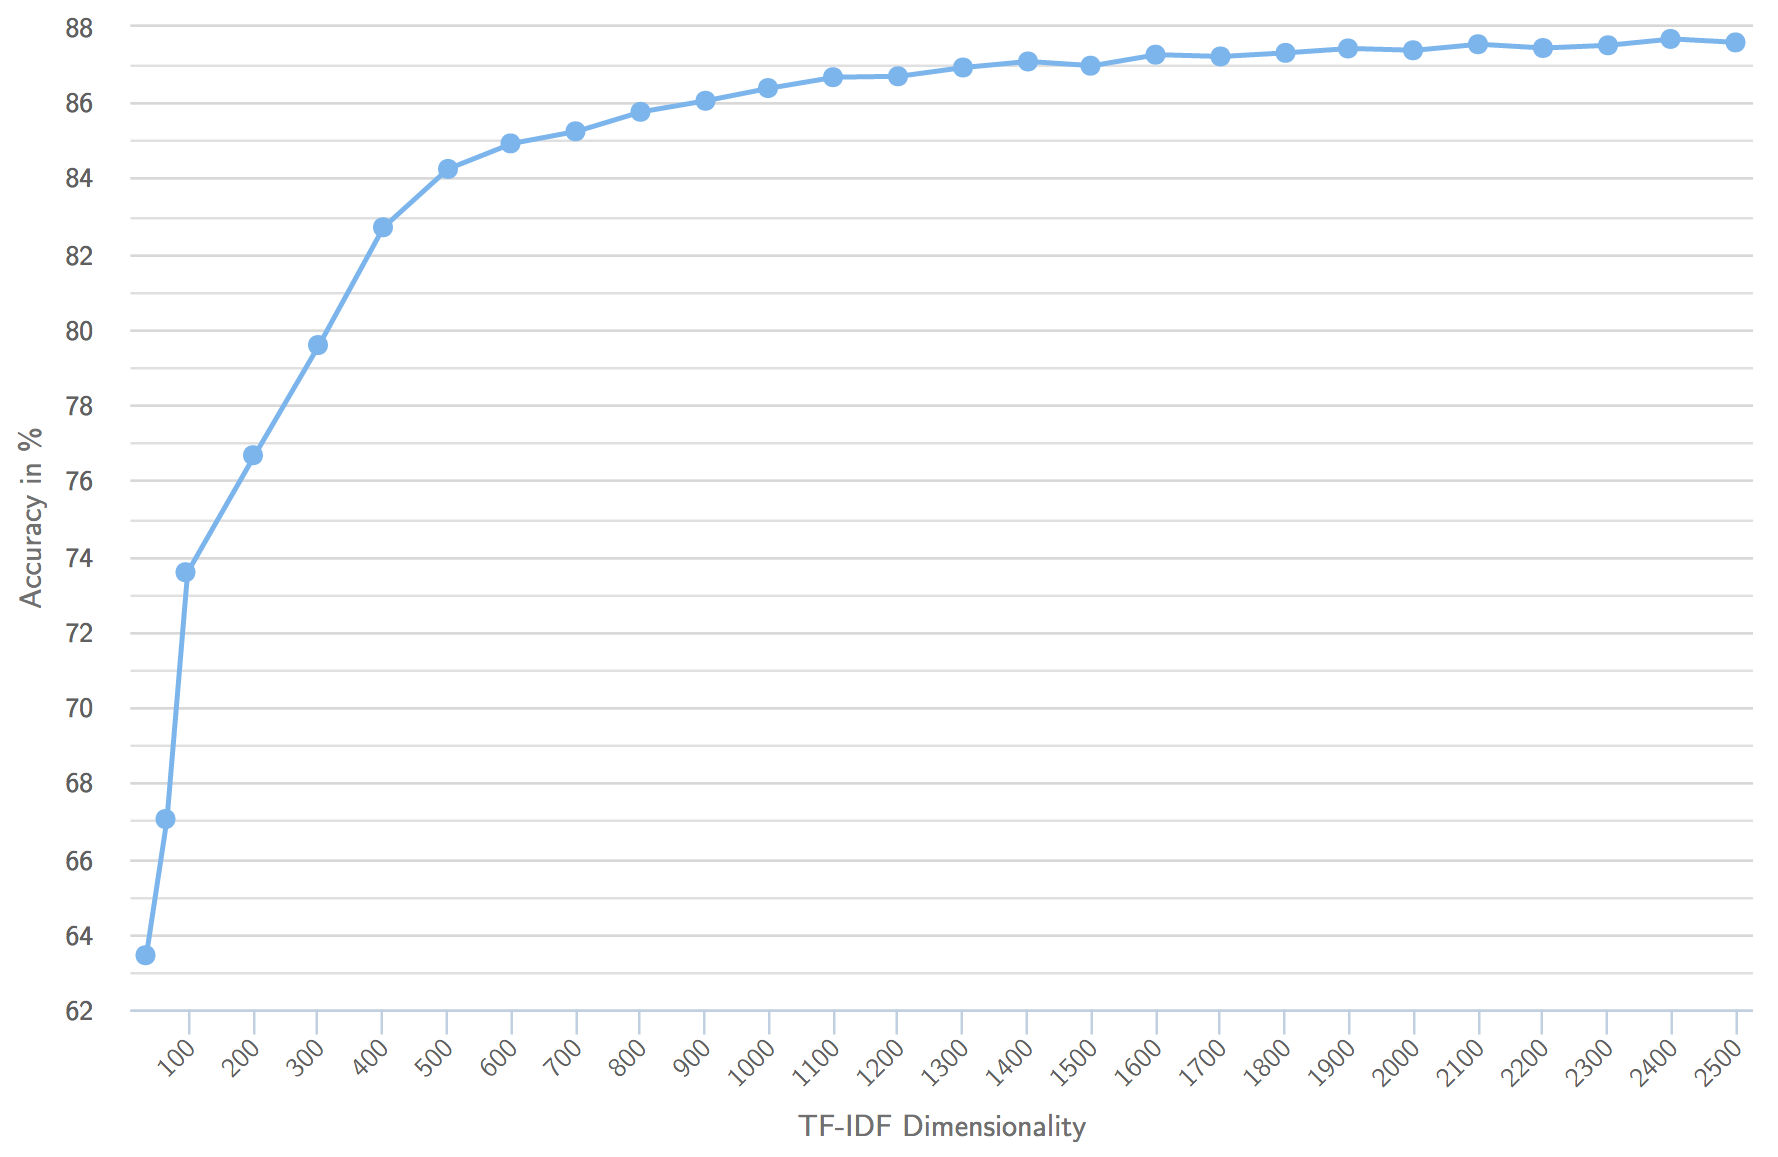
\includegraphics[width=1.0\textwidth]{5experiments/results-tfidf}
	\caption{The accuracy increases when the TF--IDF dimensionality is increased. }
	\label{fig:5:results-tfidf}
\end{figure}

When we compare the result to the values after 10 epochs of Doc2vec with 48 dimensions, see Figure~\ref{fig:5:epochs-vs-accuracy-48}, we notice that the accuracy is approximately 88.5\% in the Doc2vec case (using a total of 96 dimensions), compared to only 73.5\% accuracy in the TF--IDF case (using 96 dimensions). This means that Doc2vec outperforms TF--IDF by a substantial margin when using low-dimensional vectors.

Let us now compare TF--IDF to Doc2vec with 200 dimensions, see Figure~\ref{fig:5:epochs-vs-accuracy-200}. The accuracy for Doc2vec is approximately 90\% after multiple epochs. When we compare this to the TF--IDF score using 400 dimensions, we find an accuracy of 82.7\%. Again, Doc2vec beats the TF--IDF baseline by a considerable margin.

\subsubsection{Different HPV Implementations}

To compare the different HPV implementations against each other, the hyperparameters described in Table~\ref{tab:parameters} have been used. Because some HPV implementations clearly outperformed other implementations in multiple different configurations, instead of using multiple runs and taking the average accuracy, only one run per implementation has been conducted with this configuration. Furthermore, some HPV implementations have a slow execution speed, as we will see in~\ref{5:execution-speed-and-memory-usage}. Therefore, the additional computational cost to run multiple experiments for HPV implementations, which performed poorly, was not justified.

\begin{figure}
	\centering
	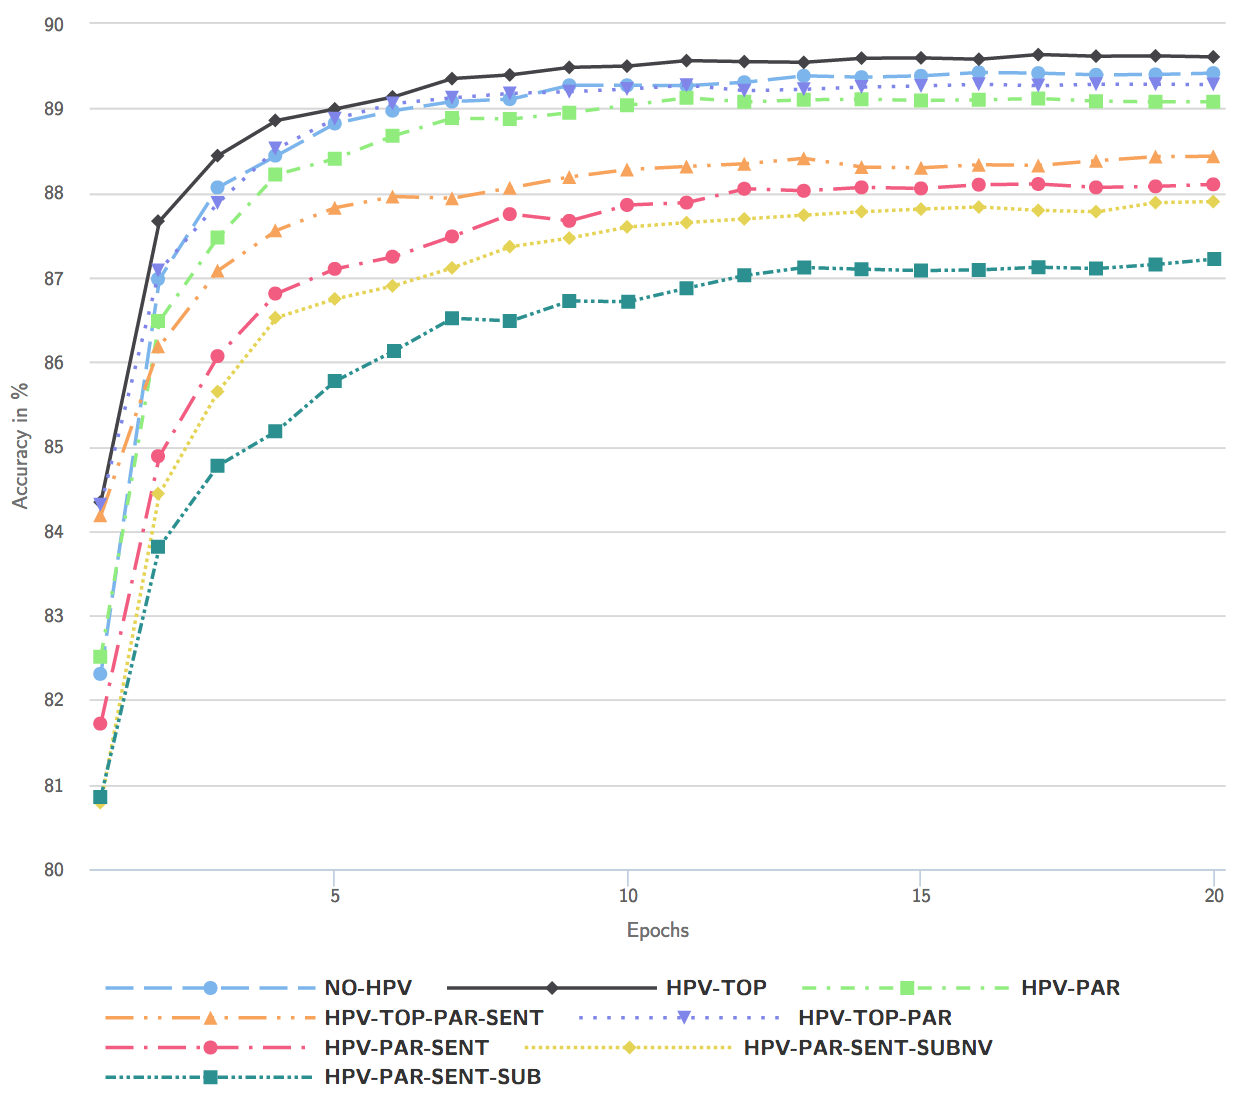
\includegraphics[width=1.0\textwidth]{5experiments/hpv-implementations}
	\caption{The accuracy increases when increasing the epochs for every HPV implementation, using a word vector dimensionality of 48. TOP boosts the accuracy significantly in the beginning. Low hierarchies do not increase the accuracy.}
	\label{fig:5:hpv-implementations}
\end{figure}

Let us now compare the different HPV implementations in Figure~\ref{fig:5:hpv-implementations}. First, we notice that after one epoch, all HPV implementations using the topic (TOP) as a hierarchy significantly outperform NO-HPV by about 2\%. Also, HPV-TOP outperforms NO-HPV here. However, this gap is not significant for all epochs, which we will see later on. Next, we notice that the more we move down in the hierarchies, the worse the accuracy develops. For example, when using paragraphs, sentences and sub-sentences, the model performs significantly worse than NO-HPV\@. Finally, when combining the topic with the lower hierarchies, the topic seems to boost the accuracy throughout all epochs, and the additional hierarchies prevent a strong increase in accuracy compared to NO-HPV\@.

The best HPV implementations from this comparison (NO-HPV, HPV-TOP, HPV-PAR) are compared in more detail in the next two subsections. HPV-TOP-PAR is left out for this comparison, because it is a combination of HPV-TOP and HPV-PAR, which both are compared against each other in the next subsections.

\subsubsection{Unrestricted Best Configuration}\label{unrestricted-best-configuration}

To compare the accuracy of the best HPV implementations to NO-HPV, the best two configurations have been chosen. The first configuration is unrestricted and thus can use an arbitrary word vector dimensionality. It uses a word vector dimensionality of 200 and the hyperparameters described in Table~\ref{tab:parameters}. The experiment has been repeated for 30 times with random initializations. Because these results represent the most important results of the empirical evaluation, significance tests have been conducted. We are using a wilcoxon signed rank test, and our hypothesis is that HPV-TOP outperforms NO-HPV, which makes it a directional test. We use a level of significance of 0.025, which corresponds to a minimum z-score of 1.960\footnote{\url{http://vassarstats.net/textbook/ch12a.html}}.

\begin{figure}
	\centering
	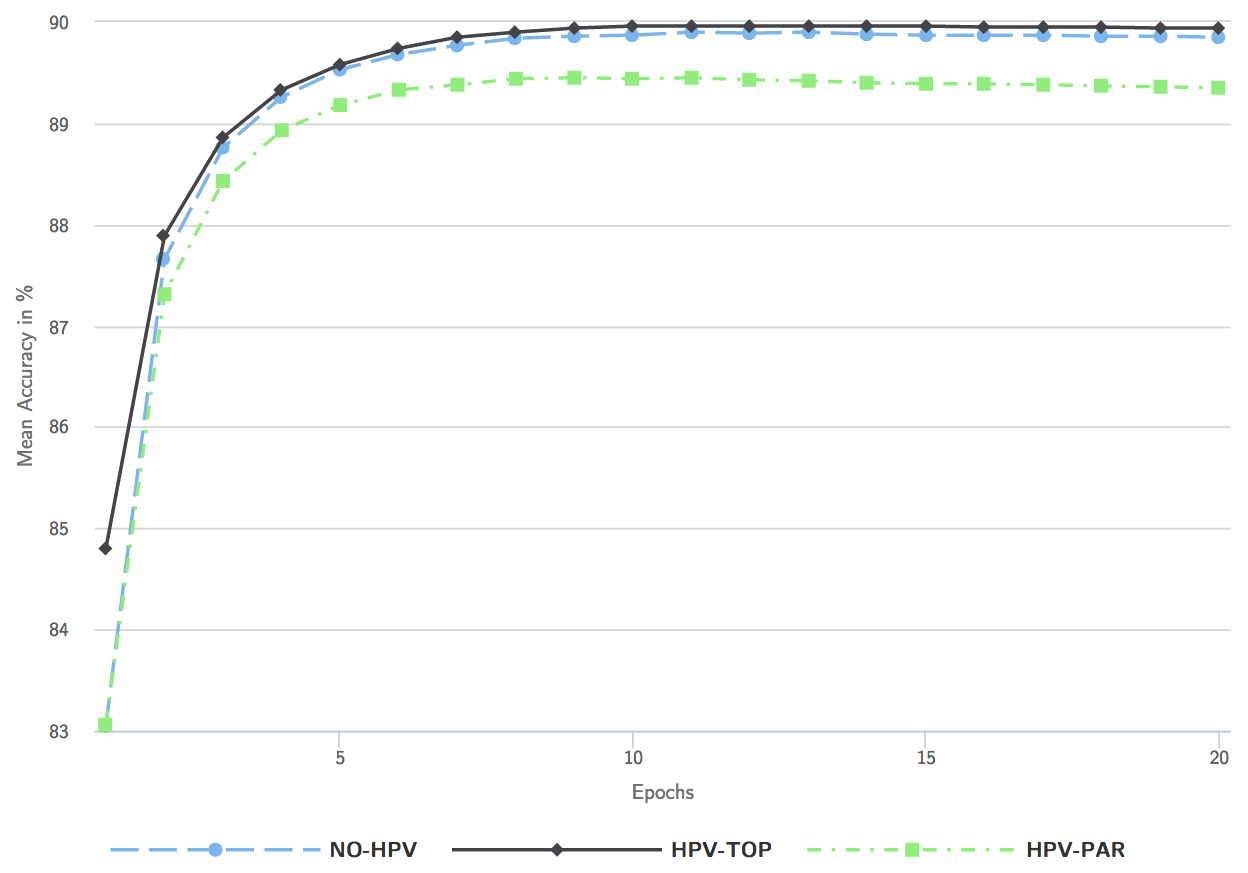
\includegraphics[width=1.0\textwidth]{5experiments/epochs-vs-accuracy-200.png}
	\caption{The mean accuracy of 30 experiments when increasing the epochs for the best configuration, using a word vector dimensionality of 200.}
	\label{fig:5:epochs-vs-accuracy-200}
\end{figure}

As we can see in Figure~\ref{fig:5:epochs-vs-accuracy-200} and Table~\ref{tab:5:epochs-vs-accuracy-200}, HPV-TOP clearly outperforms NO-HPV when only one epoch is run. When increasing the epochs, the accuracy of the prediction increases significantly for both of these implementations. HPV-TOP outperforms NO-HPV slightly by only about 0.1\%. We also notice that we reach a plateau after about 9 epochs, after which the accuracy only fluctuates marginally.

When we compare HPV-PAR to NO-HPV, we notice that after only one epoch of training, they perform very similarly. However, as the epochs progress, HPV-PAR loses steam and cannot increase the accuracy as much as NO-HPV can. Thus, NO-HPV and HPV-TOP clearly outperform HPV-PAR\@.

\begin{table}
	\centering
	\caption{The data displayed in Figure~\ref{fig:5:epochs-vs-accuracy-200}, which is the unrestricted best configuration, using word vector dimensionality of 200. The values, where HPV-TOP outperforms NO-HPV with a level of significance of 0.025, are marked with a *.}
	\label{tab:5:epochs-vs-accuracy-200}
	\begin{tabular}{lrrr}
		\toprule
		& \multicolumn{3}{c}{\emph{Accuracy [\%]}}\tabularnewline
		\emph{Epoch}& \emph{HPV-NO}& \emph{HPV-TOP}& \emph{HPV-PAR}\tabularnewline
		\midrule
		1& 83.05& *84.8& 83.06\tabularnewline
		2& 87.66& *87.89& 87.31\tabularnewline
		3& 88.76& *88.86& 88.43\tabularnewline
		4& 89.26& *89.33& 88.93\tabularnewline
		5& 89.53& 89.58& 89.18\tabularnewline
		6& 89.68& *89.74& 89.33\tabularnewline
		7& 89.77& *89.85& 89.38\tabularnewline
		8& 89.84& *89.9& 89.44\tabularnewline
		9& 89.86& *89.94& 89.45\tabularnewline
		10& 89.87& *89.96& 89.44\tabularnewline
		11& 89.9& *89.96& 89.45\tabularnewline
		12& 89.89& *89.96& 89.43\tabularnewline
		13& 89.9& 89.96& 89.42\tabularnewline
		14& 89.88& *89.96& 89.4\tabularnewline
		15& 89.87& *89.96& 89.39\tabularnewline
		16& 89.87& *89.95& 89.39\tabularnewline
		17& 89.87& *89.95& 89.38\tabularnewline
		18& 89.86& *89.95& 89.37\tabularnewline
		19& 89.86& 89.94& 89.36\tabularnewline
		20& 89.85& *89.94& 89.35\tabularnewline
		\bottomrule
	\end{tabular}
\end{table}


\subsubsection{Restricted Best Configuration}\label{restricted-best-configuration}

The second best configuration is restricted to use a low word vector dimensionality of 48 dimensions for HPV-DM and HPV-DBOW \emph{each}. For the significance tests, we apply the same strategy as in the best unrestricted configuration above, using 30 experiments with random initializations, a 0.025 level of significance, and the hypothesis that HPV-TOP outperforms NO-HPV\@.

\begin{figure}
	\centering
	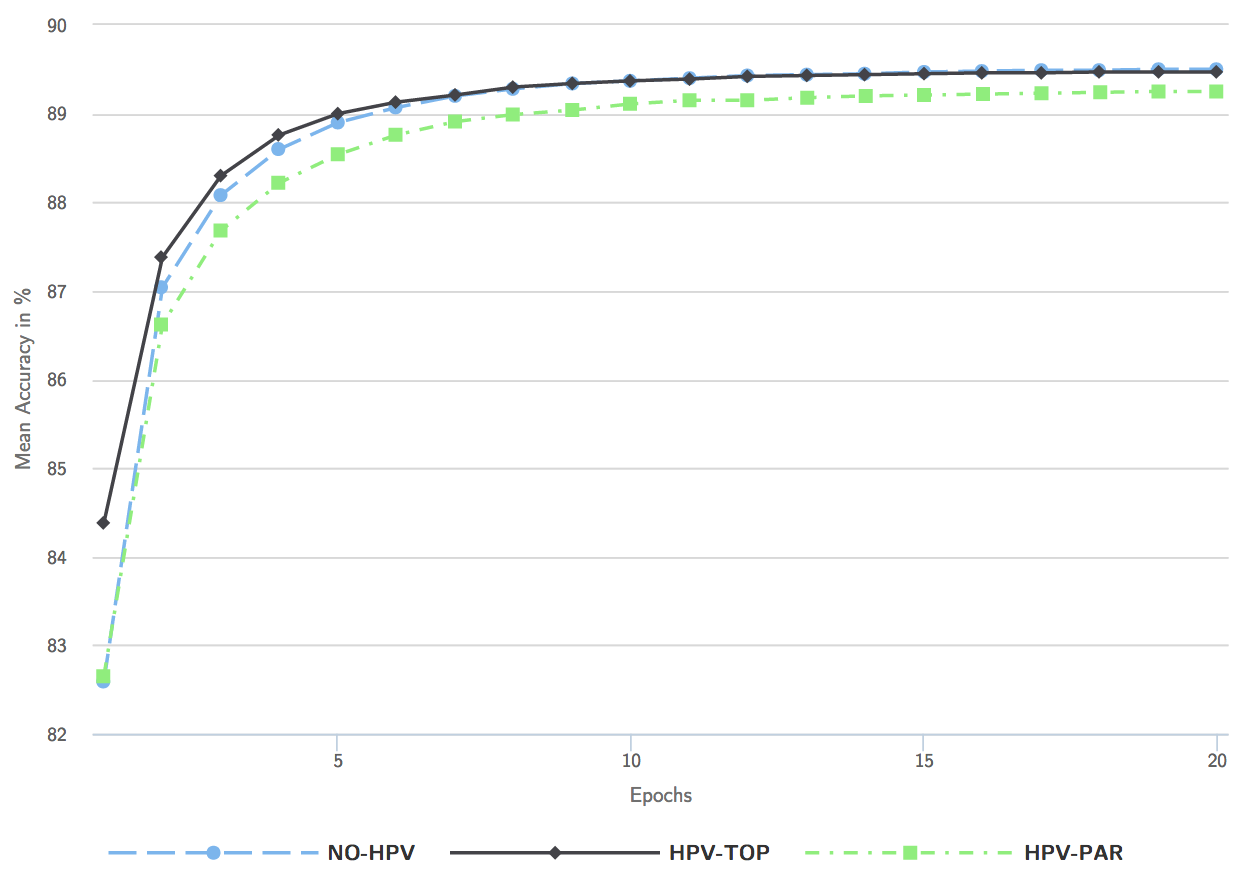
\includegraphics[width=1.0\textwidth]{5experiments/epochs-vs-accuracy-48.png}
	\caption{The mean accuracy of 30 experiments when increasing the epochs for the best configuration, using a word vector dimensionality of 48.}
	\label{fig:5:epochs-vs-accuracy-48}
\end{figure}

In Figure~\ref{fig:5:epochs-vs-accuracy-48} and Table~\ref{tab:5:epochs-vs-accuracy-48}, we again see an initial boost when using HPV-TOP compared to NO-HPV\@. However, after 8 epochs, the accuracy of HPV-TOP and NO-HPV converge. Also, in contrast to the 200 dimensional experiment, the accuracy increases slightly with further training.

For HPV-PAR, we notice similar behavior as before. After one epoch, the accuracy of HPV-PAR is the same as NO-HPV, and after that, HPV-PAR stays below NO-HPV and HPV-TOP\@.

\begin{table}
	\centering
	\caption{The data displayed in Figure~\ref{fig:5:epochs-vs-accuracy-48}, which is the restricted best configuration, using word vector dimensionality of 48. The values, where HPV-TOP outperforms NO-HPV with a level of significance of 0.025, are marked with a *. NO-HPV never outperforms HPV-TOP with a level of significance of 0.05 or lower.}
	\label{tab:5:epochs-vs-accuracy-48}
	\begin{tabular}{lrrr}
		\toprule
		& \multicolumn{3}{c}{\emph{Accuracy [\%]}}\tabularnewline
		\emph{Epoch}& \emph{HPV-NO}& \emph{HPV-TOP}& \emph{HPV-PAR}\tabularnewline
		\midrule
		1& 82.59& *84.38& 82.65\tabularnewline
		2& 87.04& *87.38& 86.62\tabularnewline
		3& 88.08& *88.3& 87.68\tabularnewline
		4& 88.6& *88.76& 88.22\tabularnewline
		5& 88.9& *89& 88.54\tabularnewline
		6& 89.07& *89.13& 88.76\tabularnewline
		7& 89.2& 89.21& 88.91\tabularnewline
		8& 89.28& 89.3& 88.99\tabularnewline
		9& 89.34& 89.34& 89.04\tabularnewline
		10& 89.37& 89.37& 89.11\tabularnewline
		11& 89.4& 89.39& 89.15\tabularnewline
		12& 89.43& 89.42& 89.15\tabularnewline
		13& 89.44& 89.43& 89.18\tabularnewline
		14& 89.45& 89.44& 89.2\tabularnewline
		15& 89.47& 89.45& 89.21\tabularnewline
		16& 89.48& 89.46& 89.22\tabularnewline
		17& 89.49& 89.46& 89.23\tabularnewline
		18& 89.49& 89.47& 89.24\tabularnewline
		19& 89.5& 89.47& 89.25\tabularnewline
		20& 89.5& 89.47& 89.25\tabularnewline
		\bottomrule
	\end{tabular}
\end{table}

\subsection{Execution Speed and Memory Usage}\label{5:execution-speed-and-memory-usage}

In this subsection, we compare the execution speed and the memory usage of the different HPV implementations. For the memory usage, we try to validate our theoretical calculation from~\ref{4:resources}.

\subsubsection{Execution Speed}

\begin{table}
	\centering
	\caption{Execution speed for training the word embeddings with a word vector dimensionality of 48 per epoch. 20 experiments per HPV implementation and model (HPV-DBOW, HPV-DM) have been conducted to calculate the average duration in seconds.}
	\label{tab:5:runtime48}
	\begin{tabular}{llrr}
		\toprule
		\emph{HPV}& \emph{Model}& \begin{tabular}[x]{@{}r@{}}\emph{Average}\\ \emph{Duration [s]}\end{tabular}& \begin{tabular}[x]{@{}r@{}}\emph{Standard}\\ \emph{Deviation}\end{tabular}\tabularnewline
		\midrule
		NO-HPV& HPV-DBOW& 23.71& 0.36\tabularnewline
		& HPV-DM& 18.01& 0.65\tabularnewline
		HPV-TOP& HPV-DBOW& 65.61& 0.61\tabularnewline
		& HPV-DM& 18.7& 0.42\tabularnewline
		HPV-TOP-PAR& HPV-DBOW& 88.85& 0.72\tabularnewline
		& HPV-DM& 27.2& 0.55\tabularnewline
		HPV-TOP-PAR-SENT& HPV-DBOW& 118.62& 9.19\tabularnewline
		& HPV-DM& 89.98& 4.3\tabularnewline
		HPV-PAR& HPV-DBOW& 45.91& 0.83\tabularnewline
		& HPV-DM& 26.98& 0.23\tabularnewline
		HPV-PAR-SENT& HPV-DBOW& 76.63& 3.56\tabularnewline
		& HPV-DM& 78.85& 0.22\tabularnewline
		HPV-PAR-SENT-SUBNV& HPV-DBOW& 111.79& 5.7\tabularnewline
		& HPV-DM& 135.13& 1.17\tabularnewline
		HPV-PAR-SENT-SUB& HPV-DBOW& 120.08& 2.84\tabularnewline
		& HPV-DM& 140.72& 1.6\tabularnewline
		\bottomrule
	\end{tabular}
\end{table}

To evaluate the execution speed, we ran 20 experiments with a word vector dimensionality of 48. The HPV implementation and the model influences the runtime substantially, which can be seen in Table \ref{tab:5:runtime48}. Furthermore, as we can see in Table \ref{tab:5:runtime48-totals}, in total, all HPV implementations are slower than the Doc2vec baseline. However, we notice that some [HPV, model] combinations, for example [NO-HPV, HPV-DM] or [HPV-TOP, HPV-DM], have comparable execution speed.

Overall, the advantage HPV gains by training ``faster'' compared to PV when using a fixed amount of epochs, it is overshadowed by the slower training speed of HPV per epoch. This effect is displayed in Figure~\ref{fig:5:epochs-vs-accuracy-200-scaled}, where the epochs are scaled according to the execution overhead.

\begin{figure}
	\centering
	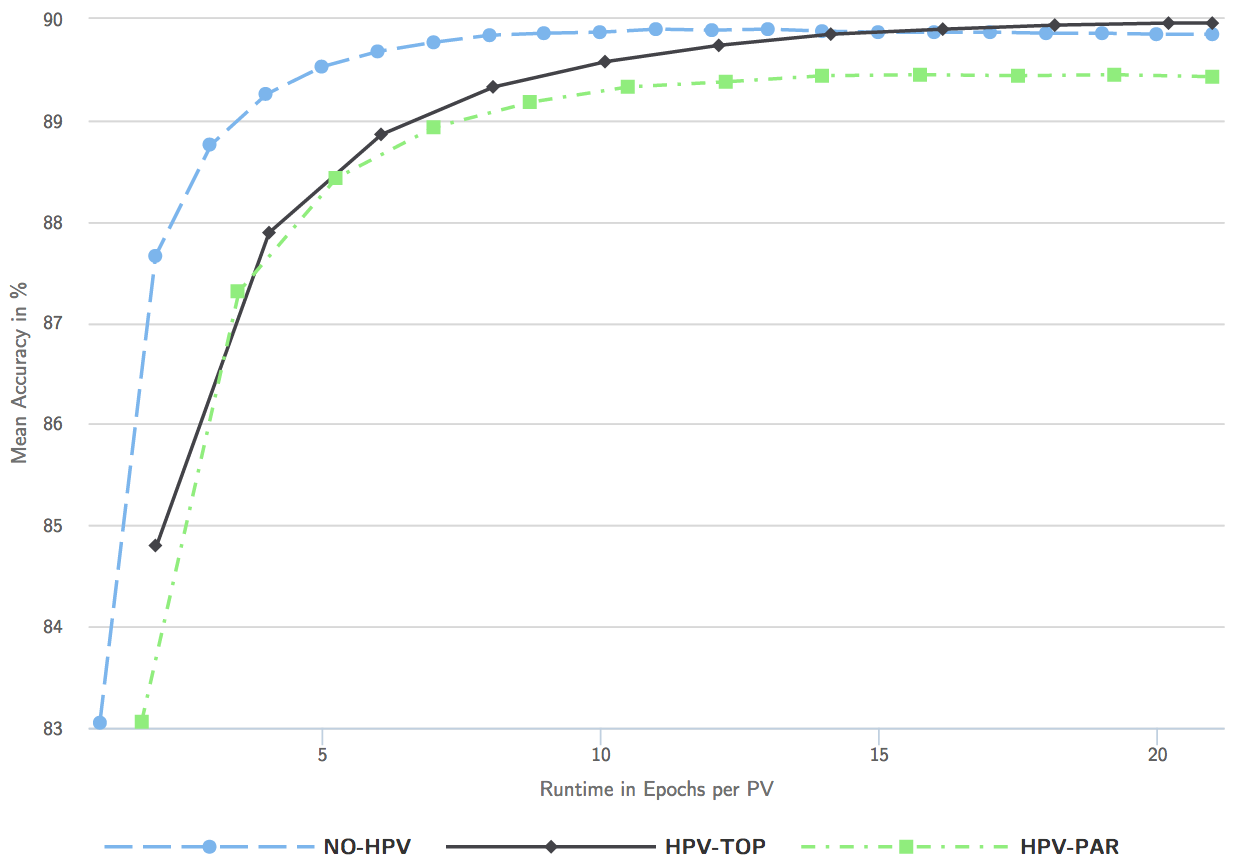
\includegraphics[width=1.0\textwidth]{5experiments/epochs-vs-accuracy-200-scaled.png}
	\caption{The mean accuracy of 30 experiments when increasing the epochs for the best configuration, using a word vector dimensionality of 200, where the epochs are scaled in relation to the execution overhead compared to NO-HPV. When considering this overhead, HPV-TOP trains considerably slower than NO-HPV, despite the initial boost in the first training epoch of HPV-TOP.}
	\label{fig:5:epochs-vs-accuracy-200-scaled}
\end{figure}

\begin{table}
	\centering
	\caption{Execution speed for training the word embeddings with a word vector dimensionality of 48 per epoch. Here, the results from Table \ref{tab:5:runtime48} are summarized.}
	\label{tab:5:runtime48-totals}
	\begin{tabular}{lrr}
		\toprule
		&  \multicolumn{2}{r}{\emph{Total Average Duration}}\tabularnewline
		\emph{HPV}& \emph{[s]} & \emph{[\%]}\tabularnewline
		\midrule
		NO-HPV& 41.72& 100\tabularnewline
		HPV-TOP& 84.31& 202\tabularnewline
		HPV-TOP-PAR& 116.05& 278\tabularnewline
		HPV-TOP-PAR-SENT& 208.60& 500\tabularnewline
		HPV-PAR& 72.89& 175\tabularnewline
		HPV-PAR-SENT& 155.48& 373\tabularnewline
		HPV-PAR-SENT-SUBNV& 246.92& 592\tabularnewline
		HPV-PAR-SENT-SUB& 260.80& 625\tabularnewline
		\bottomrule
	\end{tabular}
\end{table}


\subsubsection{Memory Usage}

Recall the formula for the additionally needed memory from \ref{4:resources}.
\begin{displaymath}
\frac{D \times G}{E \times \dim(U) +D \times K \times N}
\end{displaymath}

%todo low prio: add dim 200, add real memory

We ran the memory usage test with a window size $W=10$ and $D=E=48$ dimensions. From Table~\ref{tab:5:extracted-elements} we know $N=100'000$ documents, $Z=275$ average words per document, $dim(U)=185'957$ vocabulary size, and $K=1$ paragraph vectors per document. $G$ depends on the HPV implementation. From the results displayed in Table~\ref{tab:5:memory-usage} we notice that the formula for the memory usage overhead only fits approximately, and fails to predict the difference between HPV-PAR-SENT and HPV-PAR-SENT-SUBNV\@. At the time of writing, the source of this discrepancy is unknown, and may be caused by the implementation. Thus, it is not recommended to rely on the formula for the memory usage prediction.

\begin{table}
	\centering
	\caption{Predicted memory usage vs. measured memory usage, using a word vector dimensionality of 48. RAM is the measured ``real memory'' as reported by task\_info. It was measured during the training of the word embeddings model by using ``ps aux'' and represents a single observation.}
	\label{tab:5:memory-usage}
	\begin{tabular}{lrrrr}
		\toprule
		& & \multicolumn{3}{c}{\emph{Memory Overhead [\%]}} \tabularnewline
		& & \multicolumn{2}{c}{\emph{Serialized Model}} & \emph{RAM} \tabularnewline
		\emph{HPV}& \emph{$G$}& \emph{Predicted}& \emph{Measured}& \emph{Measured}\tabularnewline
		\midrule
		NO-HPV& 0& 0& 0& 0 \tabularnewline
		HPV-TOP& 20& 0& 0& 2 \tabularnewline
		HPV-TOP-PAR& 303468& 161& 121& 15 \tabularnewline
		HPV-TOP-PAR-SENT& 1916877& 1019& 780& 110 \tabularnewline
		HPV-PAR& 303448& 161& 121& 18 \tabularnewline
		HPV-PAR-SENT& 1916877& 1019& 780& 93 \tabularnewline
		HPV-PAR-SENT-SUBNV& 1916857& 1019& 1657& 120 \tabularnewline
		HPV-PAR-SENT-SUB& 4978237& 2647& 2039& 217 \tabularnewline
		\bottomrule
	\end{tabular}
\end{table}

%\begin{table}
%	\centering
%	\caption{toxxdo.}
%	\label{tab:xxxxxx}
%	\begin{tabular}{lr}
%		\toprule
%		\emph{AAA}& \emph{BBB}\tabularnewline
%		\midrule
%		XXX& YYY\tabularnewline
%		\bottomrule
%	\end{tabular}
%\end{table}

% \begin{tabular}[x]{@{}l@{}}TOP, PAR, SENT,\\SUB, SUBNV\end{tabular}






















